\chapter{Scheduling delle attività}
\section{Tabella di scheduling}
La tabella \ref{activity:scheduling} mostra lo scheduling delle macro-attività previsto.

\newcolumntype{C}[1]{>{\centering}p{#1}}
\begin{table}[ht]
	\centering
	\begin{tabular}{|C{2cm}|C{3cm}|C{2cm}|C{2cm}|C{2.5cm}|}
	\hline
	\textbf{Codice attività}	& \textbf{Nome attività}	& \textbf{Data inizio}	& \textbf{Data fine}	& \textbf{Codici deliverable}\tabularnewline
	\hline
	
	AC0		&	Analisi					&	15/05/2014	&	19/05/2014	& DL2\tabularnewline
	
	\hline
	
	AC1		&	Pianificazione testing			&	20/05/2014	&	4/06/2014	& DL4, DL5\tabularnewline
	
	\hline
	
	AC3		&	ODD					&	20/05/2014	&	9/07/2014	& DL3\tabularnewline
	
	\hline
	
	AC4		&	Primo incremento			&	20/05/2014	&	13/06/2014	& DL6, DL7\tabularnewline
	
	\hline
	
	AC5		&	Secondo incremento			&	 1/06/2014	&	1/07/2014	& DL8, DL9\tabularnewline
	
	\hline
	
	AC6		&	Terzo incremento			&	23/06/2014	&	7/07/2014	& DL10, DL11\tabularnewline
	
	\hline
	
	AC7		&	Management				&	28/04/2014	&	13/07/2014	& DL1, DL12\tabularnewline
	
	\hline
	\end{tabular}
	
	\caption{Scheduling delle attività}
	\label{activity:scheduling}
\end{table}

\clearpage
\section{Work Breakdown Structure (WBS)}
In questa sezione è presentata la WBS del progetto e le WBS dettagliate per documento di analisi, ODD e documentazione di testing; in particolare, per le WBS della documentazione vengono presentati due formati: l'org-chart format e l'outline format.

Nell'org-chart format vengono rappresentate le componenti principali che sono dettagliate nell'outline format per questione di spazio.
\subsection{WBS progetto}
\begin{figure}[ht]
\centering
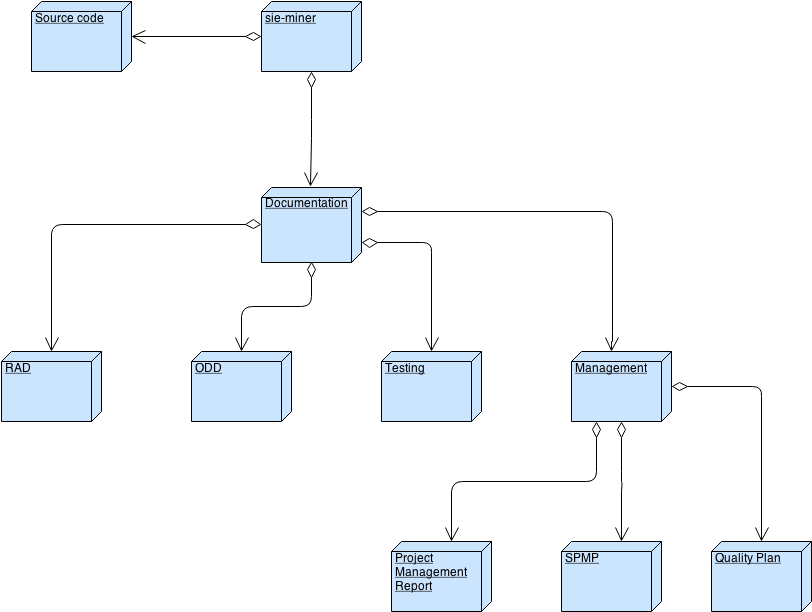
\includegraphics[width=\textwidth]{img/WBS_master.png}
\caption{WBS RepoMinerEvo} 
\end{figure}
\clearpage

% WBS Analisi ---------------------

\subsection{WBS Documento di analisi}
\begin{figure}[ht]
\centering
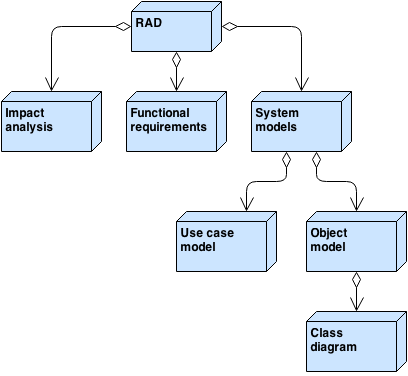
\includegraphics[width=.5\textwidth]{img/wbs_rad.png}
\caption{WBS Documento di analisi} 
\end{figure}
\textbf{WBS Documento di analisi - Outline format:}
\begin{enumerate}
\item Introduzione
\begin{enumerate}[label*=\arabic*.]
\item Scopo del sistema
\item Definizioni, acronimi, abbreviazioni
\item Panoramica
\item Sistema corrente
\end{enumerate}
\item Sistema proposto
\begin{enumerate}[label*=\arabic*.]
\item Requisiti funzionali
\end{enumerate}
\item System Model
\begin{enumerate}[label*=\arabic*.]
\item Use case models
\item Object models
\end{enumerate}
\item Impact analysis
\item Glossario
\end{enumerate}
\clearpage

% WBS ODD ---------------------
\subsection{WBS ODD}
\begin{figure}[ht]
\centering
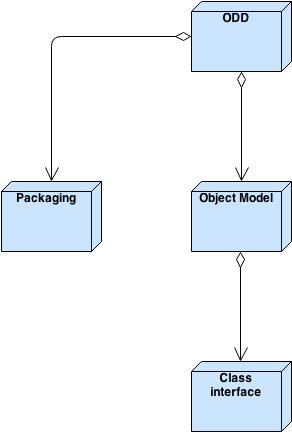
\includegraphics[width=.5\textwidth]{img/ODD.png}
\caption{WBS ODD} 
\end{figure}
\textbf{WBS ODD - Outline format:}
\begin{enumerate}
\item Introduzione
\begin{enumerate}[label*=\arabic*.]
\item Trade off dell'object design
\item Linee guida per la documentazione delle interfacce
\item Definizioni, acronimi e abbreviazioni
\item References
\end{enumerate}
\item Package
\begin{enumerate}[label*=\arabic*.]
\item Package
\item Comunicazione tra i package
\item Classi e interfacce nei package
\end{enumerate}
\item Object Model
\begin{enumerate}[label*=\arabic*.]
\item Interfaccia delle classi
\end{enumerate}
\item Glossario
\end{enumerate}
\clearpage

% WBS testing ---------------------
\subsection{WBS testing}
\begin{figure}[ht]
\centering
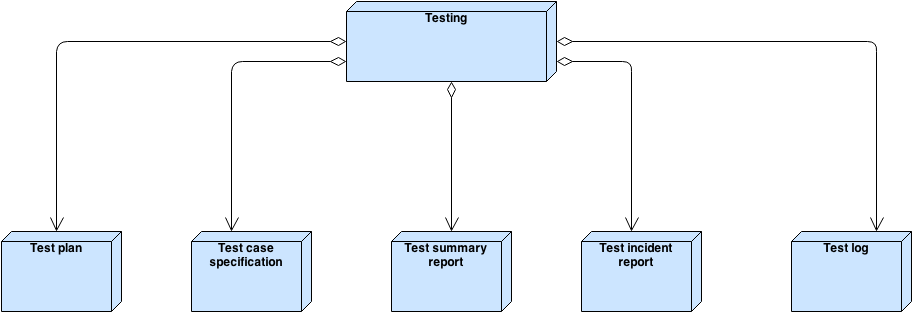
\includegraphics[width=\textwidth]{img/WBS_testing.png}
\caption{WBS Testing} 
\end{figure}
\textbf{WBS ODD - Outline format:}\\ \\
\textbf{Test Plan}:
\begin{enumerate}
\item Introduzione
\item Relazioni con altri documenti
\item Panoramica del sistema
\item Funzionalità da testare/non testare
\item Pass/Fail criteria
\item Approccio
\item Sospensione e ripristino
\item Strumenti per il testing (hardware e software)
\item Test case
\item Pianificazione del test
\end{enumerate}
\clearpage

\section{Diagramma di Gantt}
Il diagramma di Gantt riportato in figura \ref{gantMain} rappreenta lo scheduling delle attività elencate nella sezione 4.1 del presente documento
\begin{figure}[ht]
\centering
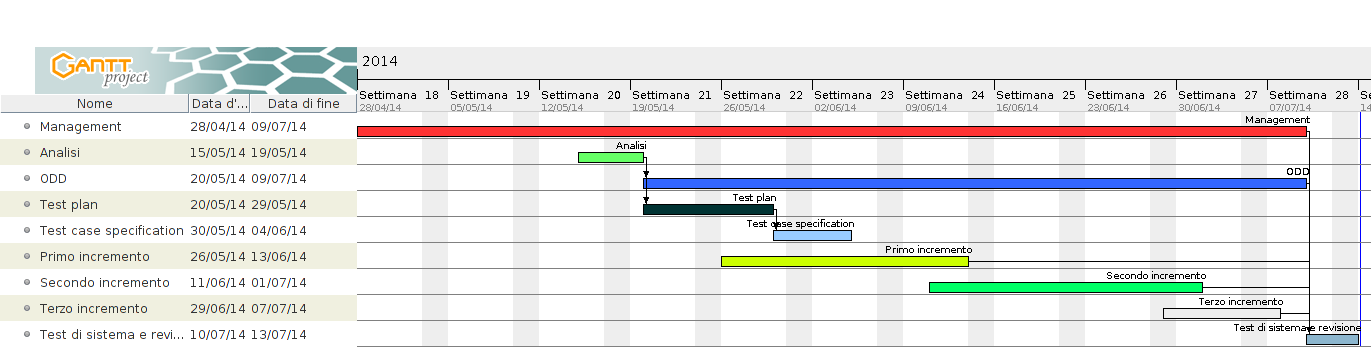
\includegraphics[width=\textwidth]{Gantt/Generic2.png} 
\caption{Diagramma di Gantt scheduling delle attività}
\label{gantMain}
\end{figure}

Di seguito le principali scandenze:
\begin{itemize}
\item 19/05/14: Consegna Documento di analisi
\item 29/05/14: Consegna Test Plan
\item 04/06/14: Consegna Test case specification
\item 13/06/14: Termine primo incremento d'implementazione
\item 01/07/14: Termine secondo incremento d'implementazione
\item 07/07/14: Termine terzo incremento d'implementazione
\item 13/07/14: Termine fase di test di sistema e revisione
\end{itemize}
